\documentclass[11pt,a4paper]{report}
\usepackage[utf8]{inputenc}
\usepackage[french]{babel}
\usepackage[T1]{fontenc}
\usepackage{amsmath}
\usepackage{amsfonts}
\usepackage{amssymb}
\usepackage{amsthm}
\usepackage{placeins}
\usepackage{makeidx}
\usepackage{svg}
\usepackage[left=2.5cm,top=2cm,right=2.5cm]{geometry}
\author{Frantzen Christian Küpper Marius}
\title{INFO-H-303 : Base de données\\
		Projet : Annuaire d'établissements horeca}
\begin{document}
\maketitle


\section*{Modèle entité-association}

\begin{figure}[h]
  \centering
  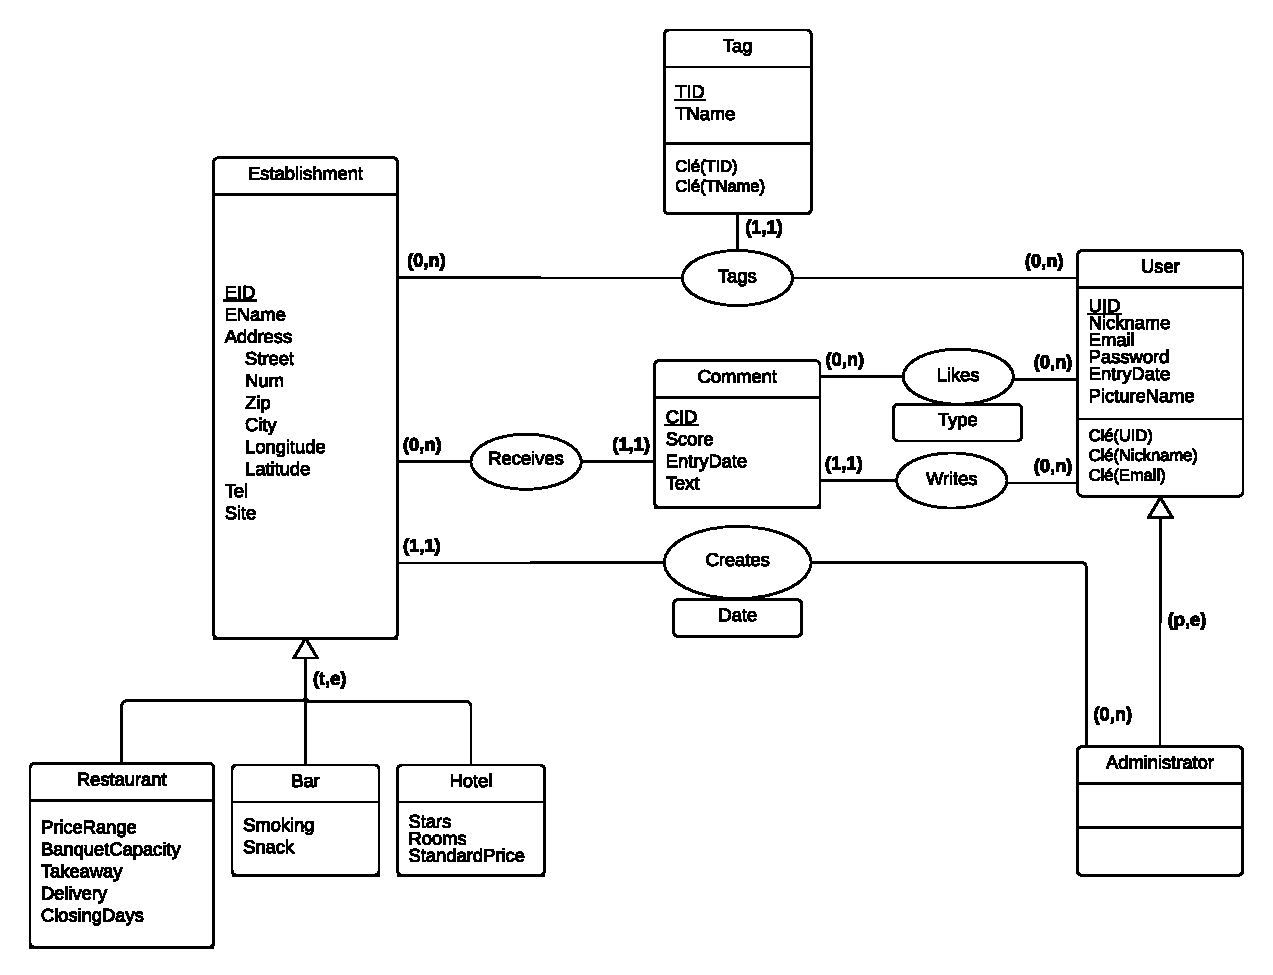
\includegraphics[width=\textwidth]{newModel.pdf}
  \caption{Modèle entité-association}
\end{figure}


\subsection*{Contraintes d'intégrité}

\begin{itemize}
\item Un \textit{User} peut commenter plusieurs fois le même \textit{Establishment} à des dates différentes. 
\item Un \textit{User} ne peut pas apposer le même \textit{Tag} plusieurs fois sur le même \textit{Establishment}.
\item L'\textit{EntryDate} d'un \textit{Adminisitrator} doit être strictement supérieure à l'\textit{EntryDate} de l'\textit{Establishment} qu'il a créé.
\item L'\textit{EntryDate} d'un \textit{Comment} doit être strictement supérieure à l'\textit{EntryDate} du User qui le fait ainsi que l'\textit{EntryDate} de l'\textit{Establishment} sur lequel il est fait. 
\item Un \textit{User} ne peut pas donner deux likes/dislikes sur un \textit{Comment}. Le \textit{Type} d'un like indique si il s'agit d'un like ou d'un dislike.
\end{itemize}
\subsection*{Remarques}
Si un \textit{Restaurant} ne veut pas organiser de banquet, il spécifie sa \textit{BanquetCapacity} comme étant 0.


\section*{Modèle relationnel}
\noindent
\textbf{Establishment}(\underline{EID},EName,Street,Num,Zip,City,Longitude,Latitude,Tel,Site,UID,EntryDate,HorecaType)
\begin{itemize}
\item UID référence User.UID (représente le createur de l'établissement)\\
\end{itemize}
\textbf{Restaurant}(\underline{EID}, PriceRange, BanquetCapacity, Takeaway, Delivery)
\begin{itemize}
\item EID référence Establishment.EID\\
\end{itemize} 
\textbf{RestaurantClosingDays}(\underline{EID}, ClosingDay, Hour)
\begin{itemize}
\item EID référence Establishment.EID\\
\end{itemize}
\textbf{Bar}(\underline{EID}, Smoking, Snack)
\begin{itemize}
\item EID référence Establishment.EID\\
\end{itemize}
\textbf{Hotel}(\underline{EID}, Stars, Rooms, StandardPrice)
\begin{itemize}
\item EID référence Establishment.EID\\
\end{itemize}
\textbf{User}(\underline{UID}, Nickname, Email, Password, EntryDate, Admin, PictureName)
\begin{itemize}
\item Nickname est unique et donc également une clé de cette relation
\item Email est unique et donc également une clé de cette relation\\
\end{itemize}
\textbf{Comment}(\underline{CID}, UID, EID, EntryDate, Score,  Text, Likes)
\begin{itemize}
\item UID référence User.UID
\item EID référence Establishment.EID
\item (UID,EID,EntryDate) est unique et donc également une clé de cette relation\\
\end{itemize}
\textbf{CommentLikes}(\underline{CID, UID}, Likes)
\begin{itemize}
\item CID référence Comment.CID
\item UID référence User.UID
\item (CID,UID) est unique et donc une clé de cette relation\\
\end{itemize}
\textbf{Tag}(\underline{TID}, TName)
\begin{itemize}
\item TName est unique et donc également une clé de cette relation\\
\end{itemize}
\textbf{EstablishmentTag}(\underline{TID, EID, UID})
\begin{itemize}
\item TID référence Tag.TID
\item EID référence Establishment.EID
\item UID référence User.UID
\item (TID,EID,UID) est unique et donc également une clé de cette relation\\
\end{itemize}


\subsection*{Remarques}
L'ajout d'une entrée dans \textit{Establishment} implique l'ajout d'une entrée dans soit \textit{Restaurant}, soit \textit{Bar} ou soit \textit{Hotel}. Les deux entrées ont le même \textit{EID}.
\subsection*{Contraintes de domaine}
\begin{itemize}
\item $User.Admin \in \{True,False\} $ (Seul les \textit{User} avec \textit{User.Admin} = True ont les droits de créer, supprimer ou modifier des \textit{Establishment}).
\item Pour les entrées dans \textit{Comment}, \textit{Comment.EntryDate > Establishment.EntryDate} et \textit{Comment.EntryDate} > \textit{User.EntryDate}
\item $Comment.Score \in \{0,1,2,3,4,5\}$
\item $Hotel.Stars \in \{0,1,2,3,4,5\}$
\item $Hotel.Rooms \in \mathbb{N}_{0}$
\item $Hotel.StandardPrice \in \mathbb{N}_{0}$
\item $Restaurant.BanquetCapacity \in \mathbb{N} $
\item $Restaurant.PriceRange \in \mathbb{N}_{0}$
\item $Restaurant.Takeaway \in \{True,False\} $
\item $Restaurant.Delivery \in \{True,False\} $
\item $RestaurantClosingDays.Hour \in \{"AM","PM","COMPLETE" \}$ (matin / après-midi / jour entier)
\item $RestaurantClosingDays.ClosingDay \in \{"MON","TUE","WED","THU","FRI","SAT","SUN" \} $
\item $Bar.Smoking \in \{True,False\} $
\item $Bar.Snack \in \{True,False\} $
\item $Comment.Likes \in \mathbb{Z} $
\item $CommentLikes.Likes \in \{True,False\} $ (like / dislike)

\end{itemize}

\section*{Script de création de la base de données}

\begin{verbatim}
CREATE DATABASE IF NOT EXISTS annuaire_horeca DEFAULT COLLATE = utf8_general_ci;

CREATE TABLE IF NOT EXISTS annuaire_horeca.users (
    uid INT(6) NOT NULL AUTO_INCREMENT,
    nickname VARCHAR(40) UNIQUE NOT NULL,
    email VARCHAR(40) DEFAULT NULL,
    password VARCHAR(70) DEFAULT NULL,
    entry_date DATETIME DEFAULT CURRENT_TIMESTAMP,
    admin BOOLEAN DEFAULT 0,
    picture_name VARCHAR(255) DEFAULT NULL,
    PRIMARY KEY (uid),
    UNIQUE(nickname),
    UNIQUE(email)
);

CREATE TABLE IF NOT EXISTS annuaire_horeca.establishments (
    eid INT(6) NOT NULL AUTO_INCREMENT ,
    ename VARCHAR(40) NOT NULL,
    street VARCHAR(40) NOT NULL,
    house_num VARCHAR(7) NOT NULL,
    zip INT(4) NOT NULL,
    city VARCHAR(20) NOT NULL,
    longitude DOUBLE(15, 7) NOT NULL,
    latitude DOUBLE(15, 7) NOT NULL,
    tel VARCHAR(20) NOT NULL,
    site VARCHAR(60),
    uid INT(6) NOT NULL,
    entry_date DATETIME DEFAULT CURRENT_TIMESTAMP,
    horeca_type ENUM('Restaurant', 'Bar', 'Hotel') NOT NULL,
    PRIMARY KEY (eid),
    FOREIGN KEY (uid) REFERENCES users(uid)
);

CREATE TABLE IF NOT EXISTS annuaire_horeca.restaurants (
    eid INT(6) NOT NULL,
    price_range INT(3) NOT NULL,
    banquet_capacity INT(3) NOT NULL,
    takeaway BOOLEAN DEFAULT 0,
    delivery BOOLEAN DEFAULT 0,
    PRIMARY KEY (eid),
    FOREIGN KEY (eid) REFERENCES establishments(eid)
);

CREATE TABLE IF NOT EXISTS annuaire_horeca.restaurant_closing_days (
    eid INT(6) NOT NULL,
    closing_day ENUM('MON', 'TUE', 'WED', 'THU', 'FRI', 'SAT', 'SUN') NOT NULL,
    hour ENUM('AM', 'PM', 'COMPLETE') NOT NULL,
    FOREIGN KEY (eid) REFERENCES establishments(eid)
);

CREATE TABLE IF NOT EXISTS annuaire_horeca.bars (
    eid INT(6) NOT NULL,
    smoking BOOLEAN DEFAULT 0,
    snack BOOLEAN DEFAULT 0,
    PRIMARY KEY (eid),
    FOREIGN KEY (eid) REFERENCES establishments(eid)
);

CREATE TABLE IF NOT EXISTS annuaire_horeca.hotels (
    eid INT(6) NOT NULL,
    stars INT(1) NOT NULL,
    rooms INT(3) NOT NULL,
    standard_price INT(3) NOT NULL,
    PRIMARY KEY (eid),
    FOREIGN KEY (eid) REFERENCES establishments(eid)
);

CREATE TABLE IF NOT EXISTS annuaire_horeca.comments (
    cid INT(6) NOT NULL AUTO_INCREMENT,
    uid INT(6) NOT NULL,
    eid INT(6) NOT NULL,
    entry_date DATETIME DEFAULT CURRENT_TIMESTAMP,
    score INT(1) NOT NULL,
    likes INT(3) DEFAULT 0,
    text TEXT NOT NULL,
    PRIMARY KEY (cid),
    FOREIGN KEY (uid) REFERENCES users(uid),
    FOREIGN KEY (eid) REFERENCES establishments(eid)
);

CREATE TABLE IF NOT EXISTS annuaire_horeca.comment_likes (
    cid INT(6) NOT NULL,
    uid INT(6) NOT NULL,
    likes BOOLEAN DEFAULT 0,
    FOREIGN KEY (uid) REFERENCES users(uid),
    FOREIGN KEY (cid) REFERENCES comments(cid)
);

CREATE TABLE IF NOT EXISTS annuaire_horeca.tags (
    tid INT(6) NOT NULL AUTO_INCREMENT,
    tname VARCHAR(35) NOT NULL,
    PRIMARY KEY (tid),
    UNIQUE (tname)
);

CREATE TABLE IF NOT EXISTS annuaire_horeca.establishment_tags (
    tid INT(6) NOT NULL,
    eid INT(6) NOT NULL,
    uid INT(6) NOT NULL,
    FOREIGN KEY (tid) REFERENCES tags(tid),
    FOREIGN KEY (uid) REFERENCES users(uid),
    FOREIGN KEY (eid) REFERENCES establishments(eid)
);
\end{verbatim}

\section*{Requêtes}

\subsection*{R1}
%----------------------------------------------------%
%----------------------------------------------------%

\noindent Tous les utilisateurs qui apprécient au moins 3 établissements que l'utilisateur "Brenda" apprécie.
\paragraph*{Calcul relationnel tuple}
\begin{align*}
\{ u | & User(u) \wedge \exists e_{1} \exists e_{2} \exists e_{3} ( Establishment(e_{1}) \wedge
Establishment(e_{2}) \wedge Establishment(e_{3}) \wedge \\ 
& e_{1} \neq e_{2} \wedge e_{1} \neq e_{3} \wedge e_{2} \neq e_{3} \wedge \exists u_{2} \exists c_{1} \exists c_{2} ( User(u_{2}) \wedge Comment(c_{1}) \wedge Comment(c_{2}) \wedge \\
& u_{2}.uid \neq u.uid \wedge u_{2}.nickname = "Brenda" \wedge \forall i \in \{1,2,3 \}(c_{1}.uid=e_{i} \wedge c_{2}.uid=e_{i} \wedge  \\
& c_{1}.uid = u.uid \wedge c_{2}.uid = u_{2}.uid \wedge  c_{1}.score \geq 4 \wedge  c_{2}.score \geq 4  )))
\}
\end{align*}
\paragraph*{Algèbre relationnelle}
\begin{align*}
& EstabsBrendaLikes \leftarrow \pi_{eid} ( ( \sigma_{score \ge 4} (Comment)) *_{uid=uid} (\sigma_{nickname = 'Brenda'} (User)) ) \\
& EstabsOthersLike \leftarrow \pi_{comment.eid, \; user.*} ( ( \sigma_{score \ge 4} (Comment)) *_{uid=uid} (\sigma_{nickname \neq 'Brenda'} (User)) )\\ 
& Result \leftarrow \sigma_{nbrLikes \ge 3} (user.*, nbrLikes \quad \gamma \quad count(eid) \; as\;  nbrLikes ( \\
& (EstabsBrendaLikes)*_{eid=eid}(EstabsOthersLike)) )
\end{align*}

\theoremstyle{plain}
\newtheorem{thm}{Theorem}
\theoremstyle{definition}
\newtheorem{defn}[thm]{Definition}

\begin{defn} L'operateur aggregate est défini comme suit: \\
\begin{math}G_1, G_2, ..., G_n \quad \gamma \quad F_1(A_1), F_2(A_2), ..., F_m(A_m) \quad (E) \end{math} \\
où \begin{math} E \end{math} est une expression d'algèbre lineaire,  \begin{math}G_1, G_2, ..., G_n \end{math} est une liste d'attributs sur lesquelles on regroupe, chaque \begin{math} F_i \end{math} est une fonction d'agrégation et chaque \begin{math} A_i \end{math} est un nom d'un attribut. \end{defn}

\paragraph*{SQL}
\begin{verbatim}
SELECT u1.*
FROM users u1, comments c1
WHERE u1.nickname != 'Brenda' AND c1.uid = u1.uid AND c1.score >= 4 AND c1.eid IN (
        SELECT DISTINCT c2.eid
        FROM comments c2, users u2
        WHERE c2.score >= 4 AND u2.nickname = 'Brenda' AND c2.uid = u2.uid
        )
GROUP BY u1.uid
HAVING COUNT( DISTINCT c1.eid ) >= 3
\end{verbatim}
\subsection*{R2}
%----------------------------------------------------%
%----------------------------------------------------%

\noindent Tous les établissements qu’apprécie au moins un utilisateur qui apprécie tous les établissements que "Brenda" apprécie.
\paragraph*{Calcul relationnel tuple}
\begin{align*}
\{e|& Establishment(e) \wedge \exists u_{1} \exists c_{1} (User(u_{1}) \wedge Comment(c_{1}) \wedge c_{1}.eid = e.eid \wedge c_{1}.uid=u_{1}.uid \wedge \\
& u_{1}.nickname \neq "Brenda" \wedge c_{1}.score \geq 4 \wedge  \exists u_{2} \exists c_{2} \exists c_{3} \exists e_{2} ( User(u_{2}) \wedge Comment(c_{2})\wedge \\
& Comment(c_{3}) \wedge Establishment(e_{2}) \wedge u_{2}.nickname = "Brenda" \wedge c_{2}.eid = u_{2}.uid \wedge \\
& c_{2}.eid = e_{2}.eid \wedge  c_{3}.eid = e_{2}.eid \wedge  c_{3}.uid = u_{1}.uid \wedge  c_{2}.uid = u_{2}.uid \wedge c_{2}.score \geq 4 \wedge c_{3}.score \geq 4
))
\}
\end{align*}
\paragraph*{Algèbre relationnelle}
\begin{align*}
& HighscoreComments \leftarrow \sigma_{score \ge 4} (Comment) \\
& EstabsBrendaLikes \leftarrow \pi_{eid} ( (\sigma_{nickname=Brenda} (User)) *_{uid=uid} (HighscoreComments) ) \\
& EstabsOthersLike \leftarrow \pi_{eid, uid} ( (\sigma_{nickname \neq Brenda} (User)) *_{uid=uid} (HighscoreComments) ) \\
& LikesSameAsBrenda \leftarrow \pi_{uid} (EstabsOthersLike / EstabsBrendaLikes) \\
& Result \leftarrow \pi_{estab.*} ((Establishment) *_{eid=eid} ((LikesSameAsBrenda) *_{uid=uid} (EstabsOthersLike)))
\end{align*}
\paragraph*{SQL}
\begin{verbatim}
SELECT DISTINCT e1.*
FROM users u1, establishments e1, comments c1
WHERE u1.uid = c1.uid AND u1.nickname != 'Brenda' AND e1.eid = c1.eid AND c1.score >= 4 AND 
      EXISTS (
          SELECT DISTINCT c2.*
          FROM comments c2 
          WHERE u1.uid = c2.uid AND c2.score >= 4 AND c2.uid = u1.uid AND e1.eid = c2.eid AND c2.eid IN (
              SELECT c2.eid
              FROM comments c3, users u2
              WHERE c3.score >= 4 AND u2.nickname = 'Brenda' AND c3.uid = u2.uid AND c3.eid = e1.eid
          )
      )
\end{verbatim}
\subsection*{R3}
%----------------------------------------------------%
%----------------------------------------------------%


Tous les établissements pour lesquels il y a au plus un commentaire.
\paragraph*{Calcul relationnel tuple}
\begin{align*}
\{ e | & Establishment(e) \wedge \exists! c_{1} ( Comment(c_{1}) \wedge c_{1}.eid = e.eid ) \vee \nexists c_{2} ( Comment(c_{2}) \wedge c_{2}.eid = e.eid )
\}
\end{align*}
\paragraph*{Algèbre relationnelle}
\begin{align*}
& 0\_Comments \leftarrow (Establishment) - ((Establishment) *_{eid=eid} (\pi_{eid} (Comment))) \\
& 1\_Comment \leftarrow ((Establishment) *_{eid=eid} \\ (\sigma_{nbrComment = 1} (eid, nbrComment \quad \gamma \quad count(cid) \; as\;  nbrComment ( \pi_{eid, cid}(Comment) )))) \\
& Result \leftarrow 0\_Comments \cup 1\_Comment
\end{align*}
\paragraph*{SQL}
\begin{verbatim}
SELECT e1.*
FROM establishments e1
WHERE NOT EXISTS (
    SELECT c1.*
    FROM comments c1
    WHERE e1.eid = c1.eid
    ) OR e1.eid IN (
        SELECT c2.eid
        FROM comments c2
        WHERE c2.eid = e1.eid
        GROUP BY e1.eid
        HAVING COUNT( c2.cid ) = 1
    )
\end{verbatim}
\subsection*{R4}
%----------------------------------------------------%
%----------------------------------------------------%


La liste des administrateurs n’ayant pas commenté tous les établissements qu’ils ont crées.
\paragraph*{Calcul relationnel tuple}
\begin{align*}
\{ u|& User(u)  \wedge u.admin =true  \wedge \exists e (Establishment(e) \wedge e.uid = u.uid  \wedge \nexists c ( Comment(c) \wedge \\
& c.eid = e.eid \wedge c.uid = u.uid )) \} 
\end{align*}
\paragraph*{Algèbre relationnelle}
\begin{align*}
& Admins \leftarrow \sigma_{admin=1} (User) \\
& AdminComments \leftarrow \pi_{uid, eid} ( (Admins) *_{uid=uid} (Comment) ) \\
& AdminCreated \leftarrow \pi_{uid, eid} ( (Admins) *_{uid=uid} (Establishment) ) \\
& Result \leftarrow \pi_{user.*} ( (User) *_{uid=uid} (AdminCreated - AdminComments) )
\end{align*}
\paragraph*{SQL}
\begin{verbatim}
SELECT u1.*
FROM users u1
WHERE u1.admin = 1 AND EXISTS (
    SELECT e1.*
    FROM establishments e1
    WHERE u1.uid = e1.uid AND NOT EXISTS (
        SELECT c1.*
        FROM comments c1
        WHERE c1.eid = e1.eid AND c1.uid = u1.uid
    )
)
\end{verbatim}

\subsection*{R5}
%----------------------------------------------------%
%----------------------------------------------------%


\paragraph*{SQL}
\begin{verbatim}
SELECT e1.*, AVG( c1.score ) AS _avg
FROM establishments e1, comments c1
WHERE e1.eid = c1.eid 
GROUP BY e1.eid 
HAVING COUNT( DISTINCT c1.cid ) >= 3
ORDER BY AVG( c1.score ) DESC
\end{verbatim}
\subsection*{R6}
%----------------------------------------------------%
%----------------------------------------------------%


\paragraph*{SQL}
\begin{verbatim}
SELECT t.*, AVG( estab_score._avg ) AS score_avg
FROM tags t
INNER JOIN (
    SELECT et2.tid AS _tid, et2.eid AS _eid, AVG(c.score) AS _avg
    FROM comments c, establishment_tags et2
    WHERE c.eid = et2.eid AND et2.tid IN (
        SELECT et3.tid AS _tid
        FROM establishment_tags et3
        GROUP BY et3.tid
        HAVING COUNT( DISTINCT et3.eid ) >= 5
    )
    GROUP BY et2.eid
) AS estab_score ON estab_score._tid = t.tid
GROUP BY t.tid 
ORDER BY AVG( estab_score._avg ) DESC
\end{verbatim}

\section*{Hypothèses}
\noindent

\begin{itemize}
\item \underline{Deux \textit{User}s ne peuvent pas avoir le même \textit{Nickname}:} L'interface doit permettre de consulter la fiche de chaque \textit{User}. Un \textit{User} qui cherche le profil de quelqu'un ne peut pas distinguer deux \textit{User}s avec le même \textit{Nickname} puisque le celui-ci est la seule donnée visible (pas d'image de profil, etc ...).
\item \underline{Un \textit{Admin} ne peut pas modifier des \textit{Comment}s ni des \textit{Tag}s:} On pourrait lui donner les droits de gestion pour vérifier qu'il n'y ait pas d'abus, mais pour le moment un \textit{Admin} ne peut que créer, modifier et enlever des \textit{Establishment}s.
\item Un \textit{User} peut donner un like ou un dislike sur un \textit{Comment}. Il ne peut pas mettre deux likes/dislikes sur un même \textit{Comment}, mais il peut annuler son like/dislike.
\item Pour les requêtes R1 et R2 on exclut l'utilisateur "Brenda" comme étant un résultat qu'on considère lors de la recherche des résultats parce que ça nous semble un peu redondant d'.
\end{itemize}

\section*{Scénario}
Étapes :
\begin{enumerate}
\item Login avec le compte de "Brenda" (mdp: "Brenda")
\item Inspection de la page de son profile
\item Recherche des établissements avec le mot 'Be'
\item Inspection du profile du Restaurant 'Mirabelle'
\item Redaction d'un commentaire pour le restaurant
\item Ajout d'un label au restaurant qui n'existait pas encore
\item Mettre un like sur un commentaire du café 'Tavernier'.
\item Logout
\item Login avec le compte de "Fred" (mdp: "Fred")
\item Ajout d'une photo de profile pour "Fred"
\item Création d'un Hotel
\item Inspection du profile du nouveau Hotel
\item Ajout d'un label au nouveau Hotel
\item Recherche et inspection du café 'Tavernier'
\item Chercher le commentaire qui a 1 like et mettre un dislike sur ce commentaire
\item Annuler le dislike en cliquant encore une fois sur le bouton 'Down'
\item Ouverture du site web du café 'Tavernier'
\item Supprimer le café Tavernier
\item Recherche et inspection du restaurant 'Chez Théo'
\item Changement de sa capacité de banquet et de ses heures d'ouvertures
\item Inspection du profile du tag 'Service au bar'
\item Logout
\item Création d'un nouveau compte
\item Login avec le nouveau compte
\item Inspection compte de 'Fred' 
\item Affichage des résultats des requêtes R1-R6
\item Faire une recherche avec l'option 'tagged by' et 'Fumeur' dans la barre de recherche
\item Logout
\end{enumerate}

\section*{Instructions d'installation de notre application}
Version de PHP utilisé : PHP 5.6.16
\begin{enumerate}
\item placer le dossier "ba3BDD" dans le dossier cible de votre serveur. ('www' pour wamp) 
\item ajouter la base de donnée en important le fichier 'Create\_Annuaire.sql' 
\item Créez un compte d'utilisateur sur votre serveur avec le nom "projetChristianMarius" et le mot de passe "123soleil"
\item Importer les données XML en visitant "localhost/ba3BDD/Models/XMLfile\_parser". Si rien ne s'affiche, tout c'est bien passé.
\item visitez "localhost/ba3BDD" et vous pouvez utiliser le site.
\end{enumerate} 
Les utilisateurs du fichier XML ont comme mot de passe leur nom d'utilisateur.
\end{document}
